\begin{figure}[htbp]
			\centering
			\resizebox{\textwidth}{!}{%
				\begin{tikzpicture}[
					trave/.style={line width=1.8pt, line cap=round, line join=round, black},
					terra/.style={line width=0.8pt, black},
					diag/.style={line width=0.90pt, black},
					nodoV/.style={circle, fill=white, draw=black,
						inner sep=0pt, minimum size=5.0pt, line width=0.80pt},
					segno/.style={circle, draw=black, fill=white, inner sep=0pt,
						minimum size=8pt, font=\tiny, line width=0.55pt},
					etlab/.style={circle, draw=black, line width=0.6pt,
						fill=white, inner sep=2pt, font=\small},
					lab/.style={font=\small},
					]
					
					\def\L{1.80}   % ℓ in cm
					\def\SEP{5.80} % separazione tra pannelli
					\def\dN{0.55}  % scala N: pℓ → 0.55 cm
					\def\dT{0.60}  % scala T: pℓ → 0.60 cm
					\def\dM{0.75}  % scala M: pℓ²/2 → 0.75 cm
					
					\def\portale{\draw[trave](0,0)--(0,\L)--(2*\L,\L)--(2*\L,0);}
					\def\cernieraA{%
						\draw[terra](0,0)--(-0.24,-0.40)--(0.24,-0.40)--cycle;
						\draw[terra](-0.34,-0.40)--(0.34,-0.40);
						\foreach \x in {-0.28,-0.16,-0.04,0.08,0.20,0.30}
						\draw[very thin](\x,-0.40)--++(-0.08,-0.11);
						\node[nodoV]at(0,0){};}
					\def\cernieraB{%
						\draw[terra](2*\L,0)--(2*\L-0.24,-0.40)--(2*\L+0.24,-0.40)--cycle;
						\draw[terra]({2*\L-0.34},-0.40)--({2*\L+0.34},-0.40);
						\foreach \x in {-0.28,-0.16,-0.04,0.08,0.20,0.30}
						\draw[very thin]({2*\L+\x},-0.40)--++(-0.08,-0.11);
						\node[nodoV]at(2*\L,0){};}
					
					%%═══ PANNELLO (a) — N₀ ══════════════════════════════════════════════
					\begin{scope}[xshift=0cm]
						%% N colonna sinistra (compressione, all'esterno = sinistra)
						\fill[gray!15](-\dN,0)--(0,0)--(0,\L)--(-\dN,\L)--cycle;
						\foreach \y in {0.15,0.30,...,1.75}
						{\draw[gray!50,very thin](-\dN,\y)--(0,\y);}
						\draw[diag](-\dN,0)--(-\dN,\L);
						\draw[diag](-\dN,0)--(0,0);
						\draw[diag](-\dN,\L)--(0,\L);
						%% N colonna destra (compressione, all'esterno = destra)
						\fill[gray!20](2*\L,0)--({2*\L+\dN},0)--({2*\L+\dN},\L)--(2*\L,\L)--cycle;
						\foreach \y in {0.15,0.30,...,1.75}
						{\draw[gray!50,very thin](2*\L,\y)--({2*\L+\dN},\y);}
						\draw[diag]({2*\L+\dN},0)--({2*\L+\dN},\L);
						\draw[diag](2*\L,0)--({2*\L+\dN},0);
						\draw[diag](2*\L,\L)--({2*\L+\dN},\L);
						%% N traverso (compressione, sotto — tratteggio verticale)
						\fill[gray!20](0,{\L-\dN/2})--(2*\L,{\L-\dN/2})--(2*\L,\L)--(0,\L)--cycle;
						\foreach \x in {0.35,0.70,...,3.50}
						{\draw[gray!50,very thin](\x,{\L-\dN/2})--(\x,\L);}
						\draw[diag](0,{\L-\dN/2})--(2*\L,{\L-\dN/2});
						%% Struttura
						\portale \cernieraA \cernieraB
						\node[nodoV]at(\L,\L){};
						%% Segni ±
						\node[segno]at({-\dN/2},{\L*0.50}){$-$};
						\node[segno]at({2*\L+\dN/2},{\L*0.50}){$-$};
						\node[segno]at({0.5*\L},{\L-\dN/4}){$-$};
						\node[segno]at({1.5*\L},{\L-\dN/4}){$-$};
						%% Valori
						\node[left=0.04,lab]at(-\dN,{\L*0.50}){$p\ell$};
						\node[right=0.04,lab]at({2*\L+\dN},{\L*0.50}){$p\ell$};
						\node[below=0.04,lab]at(\L,{\L-\dN/2}){$\tfrac{p\ell}{2}$};
						%% Etichette nodi
						\node[right,lab]at(0,0){$A$};
						\node[left,lab]at(2*\L,0){$B$};
						\node[above,lab]at(0,\L){$C$};
						\node[above,lab]at(2*\L,\L){$D$};
						\node[above,lab]at(\L,\L){$M$};
						%% Label cerchiata al centro del portale
						\node[etlab]at(\L,{0}){$N_0$};
					\end{scope}
					
					%%═══ PANNELLO (b) — T₀ ══════════════════════════════════════════════
					\begin{scope}[xshift=\SEP cm]
						%% T colonna sinistra (T = −pℓ/2, esterno = sinistra)
						\fill[gray!15]({-\dT/2},0)--(0,0)--(0,\L)--({-\dT/2},\L)--cycle;
						\foreach \y in {0.15,0.30,...,1.75}
						{\draw[gray!50,very thin]({-\dT/2},\y)--(0,\y);}
						\draw[diag]({-\dT/2},0)--({-\dT/2},\L);
						\draw[diag]({-\dT/2},0)--(0,0);
						\draw[diag]({-\dT/2},\L)--(0,\L);
						%% T colonna destra (T = +pℓ/2, esterno = destra)
						\fill[gray!15](2*\L,0)--({2*\L+\dT/2},0)--({2*\L+\dT/2},\L)--(2*\L,\L)--cycle;
						\foreach \y in {0.15,0.30,...,1.75}
						{\draw[gray!50,very thin](2*\L,\y)--({2*\L+\dT/2},\y);}
						\draw[diag]({2*\L+\dT/2},0)--({2*\L+\dT/2},\L);
						\draw[diag](2*\L,0)--({2*\L+\dT/2},0);
						\draw[diag](2*\L,\L)--({2*\L+\dT/2},\L);
						%% T traverso parte positiva (C→M, sopra — tratteggio verticale)
						\fill[gray!15](0,\L)--(0,{\L+\dT})--(\L,\L)--cycle;
						\begin{scope}
							\clip(0,\L)--(0,{\L+\dT})--(\L,\L)--cycle;
							\foreach \x in {0.25,0.50,...,1.75}
							{\draw[gray!50,very thin](\x,{\L-0.1})--(\x,{\L+\dT+0.1});}
						\end{scope}
						\draw[diag](0,{\L+\dT})--(\L,\L);
						\draw[diag](0,\L)--(0,{\L+\dT});
						%% T traverso parte negativa (M→D, sotto — tratteggio verticale)
						\fill[gray!15](\L,\L)--(2*\L,{\L-\dT})--(2*\L,\L)--cycle;
						\begin{scope}
							\clip(\L,\L)--(2*\L,{\L-\dT})--(2*\L,\L)--cycle;
							\foreach \x in {1.95,2.20,...,3.55}
							{\draw[gray!50,very thin](\x,{\L-\dT-0.1})--(\x,{\L+0.1});}
						\end{scope}
						\draw[diag](\L,\L)--(2*\L,{\L-\dT});
						\draw[diag](2*\L,{\L-\dT})--(2*\L,\L);
						%% Struttura
						\portale \cernieraA \cernieraB
						\node[nodoV]at(\L,\L){};
						%% Segni ±
						\node[segno]at({-\dT/4},{\L*0.50}){$-$};
						\node[segno]at({2*\L+\dT/4},{\L*0.50}){$+$};
						\node[segno]at({0.28*\L},{\L+0.22}){$+$};
						\node[segno]at({1.72*\L},{\L-0.22}){$-$};
						%% Valori
						\node[left=0.04,lab]at({-\dT/2},{\L*0.50}){$\tfrac{p\ell}{2}$};
						\node[right=0.04,lab]at({2*\L+\dT/2},{\L*0.50}){$\tfrac{p\ell}{2}$};
						\node[left=0.04,lab]at(0,{\L+\dT}){$p\ell$};
						\node[right=0.04,lab]at({2*\L-0.60},{\L-\dT-0.2}){$p\ell$};
						%% Etichette nodi
						\node[right,lab]at(0,0){$A$};
						\node[left,lab]at(2*\L,0){$B$};
						\node[above left,lab]at(0,\L){$C$};
						\node[above,lab]at(2*\L,\L){$D$};
						\node[above,lab]at(\L,\L){$M$};
						%% Label cerchiata al centro del portale
						\node[etlab]at(\L,{0}){$T_0$};
					\end{scope}
					
					%%═══ PANNELLO (c) — M₀ ══════════════════════════════════════════════
					\begin{scope}[xshift={2*\SEP cm}]
						%% M colonna sinistra (lineare 0→−pℓ²/2, a sinistra — tratteggio orizzontale)
						\fill[gray!15](0,0)--(-\dM,\L)--(0,\L)--cycle;
						\begin{scope}
							\clip(0,0)--(-\dM,\L)--(0,\L)--cycle;
							\foreach \y in {0.15,0.30,...,1.75}
							{\draw[gray!50,very thin]({-\dM-0.1},\y)--(0.1,\y);}
						\end{scope}
						\draw[diag](0,0)--(-\dM,\L);
						\draw[diag](-\dM,\L)--(0,\L);
						%% M colonna destra (lineare 0→−pℓ²/2, a destra — tratteggio orizzontale)
						\fill[gray!15](2*\L,0)--({2*\L+\dM},\L)--(2*\L,\L)--cycle;
						\begin{scope}
							\clip(2*\L,0)--({2*\L+\dM},\L)--(2*\L,\L)--cycle;
							\foreach \y in {0.15,0.30,...,1.75}
							{\draw[gray!50,very thin](2*\L-0.1,\y)--({2*\L+\dM+0.1},\y);}
						\end{scope}
						\draw[diag](2*\L,0)--({2*\L+\dM},\L);
						\draw[diag]({2*\L+\dM},\L)--(2*\L,\L);
						%% M traverso (parabolico sopra — tratteggio verticale)
						\fill[gray!15](0,\L)--(0,{\L+\dM})
						-- plot[domain=0:2*\L,samples=40]({\x},{\L+\dM*((\x-\L)/\L)^2})
						-- (2*\L,\L)--cycle;
						\begin{scope}
							\clip(0,\L)--(0,{\L+\dM})
							-- plot[domain=0:2*\L,samples=40]({\x},{\L+\dM*((\x-\L)/\L)^2})
							-- (2*\L,\L)--cycle;
							\foreach \x in {0.25,0.50,...,3.55}
							{\draw[gray!50,very thin](\x,{\L-0.1})--(\x,{\L+\dM+0.1});}
						\end{scope}
						\draw[diag] plot[domain=0:2*\L,samples=40]
						({\x},{\L+\dM*((\x-\L)/\L)^2});
						\draw[diag](0,\L)--(0,{\L+\dM});
						\draw[diag](2*\L,\L)--(2*\L,{\L+\dM});
						%% Archetti di continuità in C e D (quarto di cerchio, raggio \dM)
						\draw[diag](-\dM,\L) arc(180:90:\dM);      % C: sinistra → alto
						\draw[diag](2*\L,{\L+\dM}) arc(90:0:\dM);  % D: alto → destra
						%% Struttura
						\portale \cernieraA \cernieraB
						\node[nodoV]at(\L,\L){};
						%% Valori
						\node[left=0.04,lab]at(-\dM,\L){$\tfrac{p\ell^2}{2}$};
						\node[right=0.04,lab]at({2*\L+\dM},\L){$\tfrac{p\ell^2}{2}$};
						%% Etichette nodi
						\node[below left,lab]at(0,0){$A$};
						\node[below right,lab]at(2*\L,0){$B$};
						\node[left,lab]at(0,{\L+0.20}){$C$};
						\node[right,lab]at(2*\L,{\L+0.20}){$D$};
						\node[below=0.04,lab]at(\L,\L){$M$};
						%% Label cerchiata al centro del portale
						\node[etlab]at(\L,{0}){$M_0$};
					\end{scope}
					
				\end{tikzpicture}
			}%
			\caption{Problema~$0$: diagrammi di $N_0$, $T_0$ e $M_0$
				sul portale a tre cerniere sotto il carico uniforme~$p$.
				Gli archetti in $C$ e $D$ indicano la continuità del momento
				flettente ai nodi rigidi.}
			\label{fig:portale_problema0}
		\end{figure}
